
% TikZ Plots for E-Methanol MILP Optimization Thesis
% =================================================
% 
% Include these plots in your thesis using:
% \input{path/to/tikz_plots/plot_name.tex}
%
% Required packages in your thesis preamble:
% \usepackage{tikz}
% \usepackage{pgfplots}
% \usetikzlibrary{shapes.geometric,arrows,positioning,calc}
% \pgfplotsset{compat=1.17}

% cost_comparison
% ==============================
\begin{figure}[htbp]
\centering
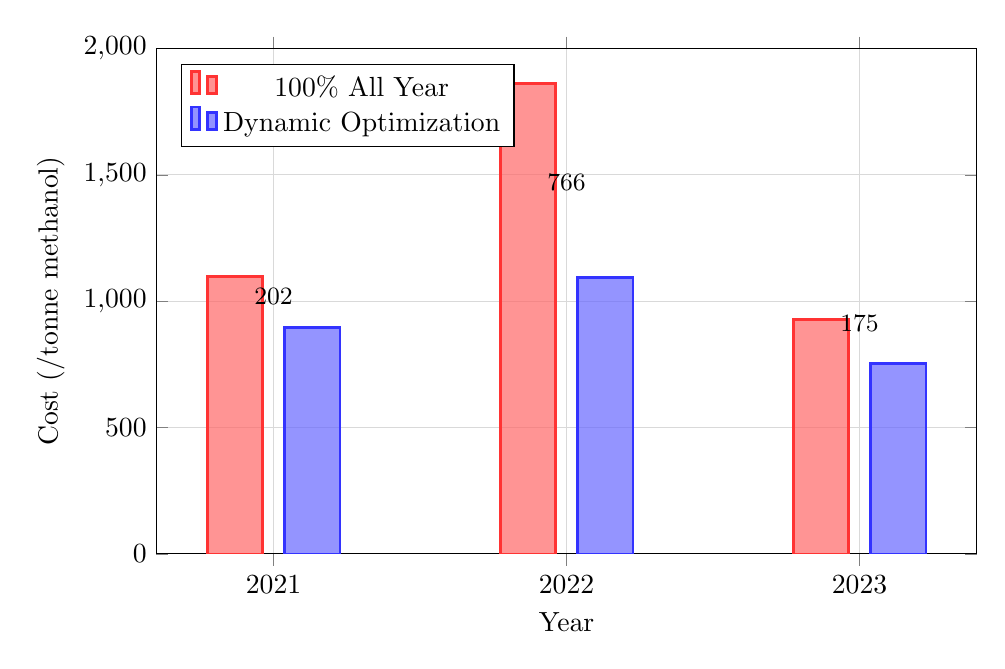
\begin{tikzpicture}
\begin{axis}[
    width=12cm,
    height=8cm,
    xlabel={Year},
    ylabel={Cost (\euro/tonne methanol)},
    ymin=0,
    ymax=2000,
    xtick=data,
    symbolic x coords={2021,2022,2023},
    legend pos=north west,
    grid=major,
    grid style={gray!30},
    bar width=20pt,
    ybar=8pt,
    enlarge x limits=0.2,
    every axis plot/.append style={
        fill opacity=0.7,
        draw opacity=1,
        line width=1pt
    }
]

% 100% All Year Strategy
\addplot[
    fill=red!60,
    draw=red!80,
] coordinates {
    (2021,1099)
    (2022,1860)
    (2023,927)
};

% Dynamic Optimization Strategy
\addplot[
    fill=blue!60,
    draw=blue!80,
] coordinates {
    (2021,897)
    (2022,1094)
    (2023,752)
};

% Add savings annotations
\node at (axis cs:2021,950) [anchor=south] {\small \euro202};
\node at (axis cs:2022,1400) [anchor=south] {\small \euro766};
\node at (axis cs:2023,840) [anchor=south] {\small \euro175};

\legend{100\% All Year, Dynamic Optimization}

\end{axis}
\end{tikzpicture}
\caption{Cost comparison between continuous operation and dynamic optimization strategies across different years}
\label{fig:cost-comparison}
\end{figure}


% operational_profile
% ==============================
\begin{figure}[htbp]
\centering
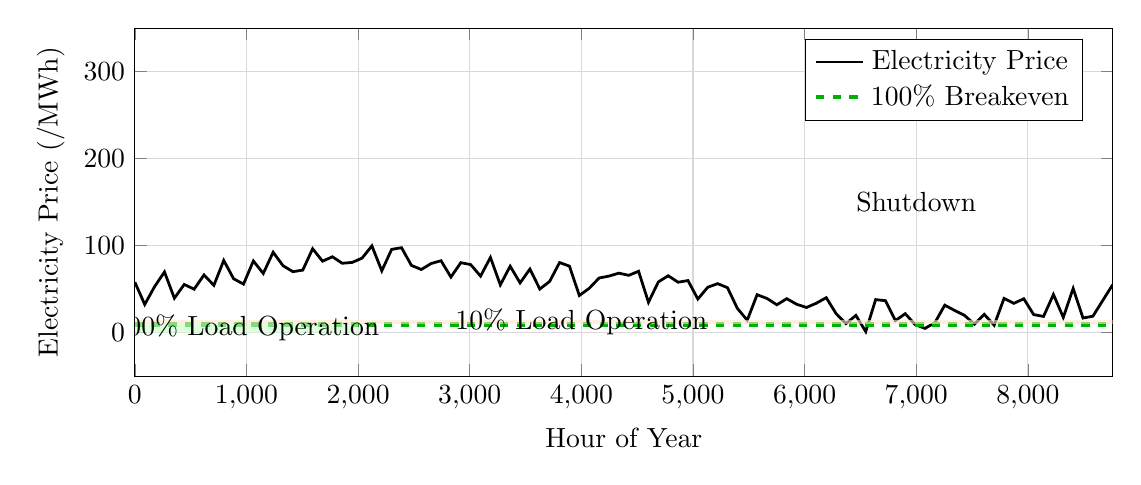
\begin{tikzpicture}
\begin{axis}[
    width=14cm,
    height=6cm,
    xlabel={Hour of Year},
    ylabel={Electricity Price (\euro/MWh)},
    xmin=0,
    xmax=8760,
    ymin=-50,
    ymax=350,
    grid=major,
    grid style={gray!30},
    legend pos=north east,
    every axis plot/.append style={line width=1pt}
]

% Simplified price profile (representative data)
\addplot[
    color=black,
    mark=none,
    samples=100,
    domain=0:8760,
] {50 + 30*sin(deg(x/1460)) + 20*rand};

% Breakeven lines
\addplot[
    color=green!70!black,
    dashed,
    line width=1.5pt,
    domain=0:8760,
] {9.42};

% Operation zones (simplified)
\fill[green!20, opacity=0.6] (axis cs:0,0) rectangle (axis cs:2000,9.42);
\fill[orange!20, opacity=0.6] (axis cs:0,9.42) rectangle (axis cs:8760,15);

\node at (axis cs:1000,5) {100\% Load Operation};
\node at (axis cs:4000,12) {10\% Load Operation};
\node at (axis cs:7000,150) {Shutdown};

\legend{Electricity Price, 100\% Breakeven}

\end{axis}
\end{tikzpicture}
\caption{Operational strategy based on electricity price thresholds}
\label{fig:operational-profile}
\end{figure}


% savings_breakdown
% ==============================
\begin{figure}[htbp]
\centering
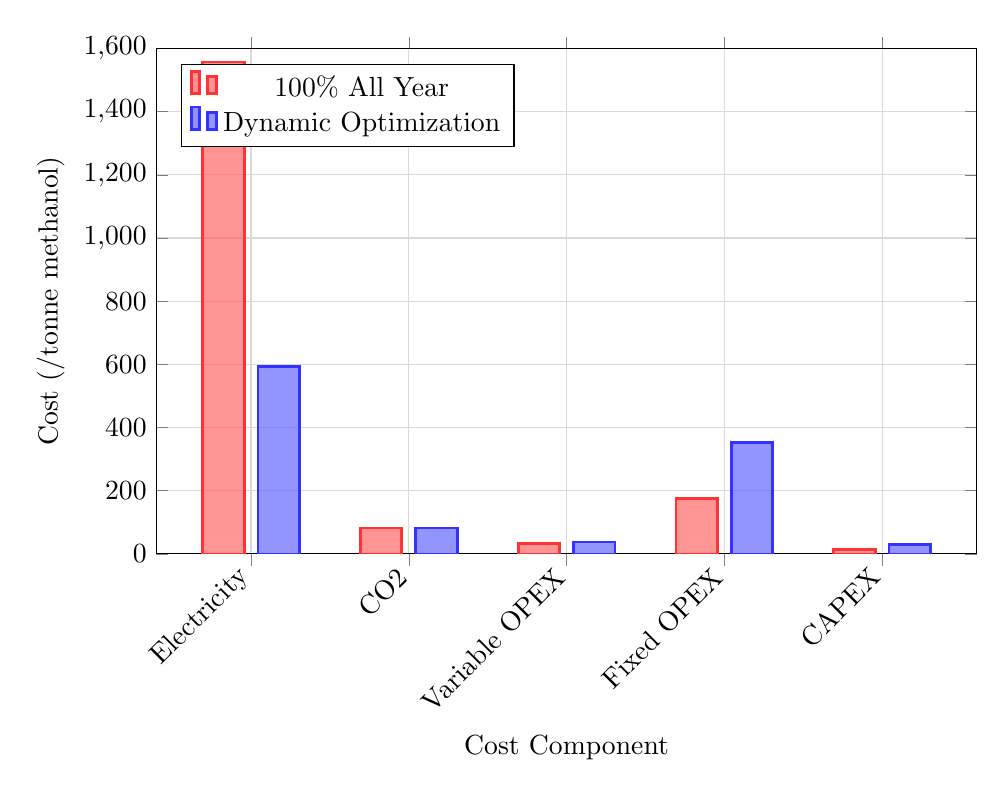
\begin{tikzpicture}
\begin{axis}[
    width=12cm,
    height=8cm,
    xlabel={Cost Component},
    ylabel={Cost (\euro/tonne methanol)},
    ymin=0,
    ymax=1600,
    xtick=data,
    symbolic x coords={Electricity,CO2,Variable OPEX,Fixed OPEX,CAPEX},
    legend pos=north west,
    grid=major,
    grid style={gray!30},
    bar width=15pt,
    ybar=5pt,
    enlarge x limits=0.15,
    x tick label style={rotate=45,anchor=east},
    every axis plot/.append style={
        fill opacity=0.7,
        draw opacity=1,
        line width=1pt
    }
]

% 2022 data (highest electricity prices) - 100% strategy
\addplot[
    fill=red!60,
    draw=red!80,
] coordinates {
    (Electricity,1557)
    (CO2,82)
    (Variable OPEX,32)
    (Fixed OPEX,176)
    (CAPEX,15)
};

% 2022 data - Dynamic strategy
\addplot[
    fill=blue!60,
    draw=blue!80,
] coordinates {
    (Electricity,593)
    (CO2,82)
    (Variable OPEX,38)
    (Fixed OPEX,352)
    (CAPEX,29)
};

\legend{100\% All Year, Dynamic Optimization}

\end{axis}
\end{tikzpicture}
\caption{Cost breakdown comparison for 2022 data (highest electricity price year)}
\label{fig:cost-breakdown}
\end{figure}


% process_flow
% ==============================
\begin{figure}[htbp]
\centering
\begin{tikzpicture}[
    node distance=2cm,
    auto,
    block/.style={rectangle, draw, rounded corners, text width=2.5cm, text centered, minimum height=1.5cm},
    input/.style={block, fill=blue!20},
    process/.style={block, fill=green!20},
    output/.style={block, fill=orange!20},
    decision/.style={diamond, draw, text width=1.8cm, text centered, minimum height=1.5cm, fill=yellow!20},
    arrow/.style={-{Stealth[length=3mm]}, thick}
]

% Input nodes
\node[input] (elec) {Electricity\\Price Signal};
\node[input, below=of elec] (co2) {CO$_2$\\Supply};
\node[input, below=of co2] (water) {Water\\Supply};

% Decision node
\node[decision, right=3cm of elec] (optimizer) {MILP\\Optimizer};

% Process nodes
\node[process, right=3cm of optimizer] (electrolyzer) {Electrolyzer\\(0-100\%)};
\node[process, below=of electrolyzer] (synthesis) {Methanol\\Synthesis};

% Output nodes
\node[output, right=2cm of electrolyzer] (h2) {H$_2$\\Production};
\node[output, right=2cm of synthesis] (methanol) {Methanol\\Product};

% Control signals
\node[above=0.5cm of electrolyzer] (control) {\footnotesize Load Level};

% Arrows
\draw[arrow] (elec) -- (optimizer);
\draw[arrow] (optimizer) -- (electrolyzer);
\draw[arrow] (optimizer) |- (control);
\draw[arrow] (co2) -| (synthesis);
\draw[arrow] (water) -| (electrolyzer);
\draw[arrow] (electrolyzer) -- (h2);
\draw[arrow] (electrolyzer) -- (synthesis);
\draw[arrow] (synthesis) -- (methanol);

% Labels
\node[below=0.2cm of optimizer] {\footnotesize Binary Decision};
\node[right=0.2cm of control] {\footnotesize 100\% or 10\%};

\end{tikzpicture}
\caption{E-methanol plant with MILP optimization control system}
\label{fig:process-flow}
\end{figure}
